\documentclass{beamer}
\usepackage{ctex}
\setCJKmainfont{思源宋体} % 设置缺省中文字体
\usepackage{fourier}     % 配置西文与数学字体

\usepackage{fontawesome5} % 矢量图标

\hypersetup{pdfcreator=TeX,
pdfpagemode = FullScreen,
}

\mode<presentation>
{
  \usetheme{XJTU}
  \useinnertheme{rounded}
  \usefonttheme{serif}
}

\title[Tech Lec]{钱院学辅技术讲座}
\subtitle{第一讲:网页设计与Markdown文档}

\author[xjtu-blacksmith]{黑山雁}

\institute[Xi'an Jiaotong University]
{
  西安交通大学
}

\date{\today}

\subject{技术,讲座}

\AtBeginSection[]
{
  \begin{frame}<beamer>{目录}
    \tableofcontents[currentsection]
  \end{frame}
}

%\beamerdefaultoverlayspecification{<+->}


\begin{document}
\begin{frame}
\maketitle
\end{frame}

\begin{frame}{目录}
    \tableofcontents
\end{frame}

\section{网页设计}
\begin{frame}{网页设计}
\begin{block}{定义 Definition}
A \textbf{web page} (also written as \textbf{webpage}) is a document that is
suitable to act as a web resource on the World Wide Web \ldots Typical web pages
are hypertext documents which contain hyperlinks, often referred to as \emph{links},
for browsing to other web pages.

\raggedleft --- Wikipedia: \emph{Web page}
\end{block}

\begin{itemize}
    \item 超文本内容(hypertext contents)
    \item 超链接(hyperlinks, links)
    \item 样式表(style sheets)
    \item 脚本代码(scripts)
\end{itemize}
\end{frame}

\subsection{从「三剑客」说起}
\begin{frame}{从「三剑客」说起}{Macromedia 的昔日荣光}
\centerline{
\includegraphics[width=0.4\textwidth]{pic/macromedia.png}}

\begin{itemize}
    \item 老「三剑客」:Dreamweaver、Fireworks、Flash
    \begin{itemize}
        \item Dreamweaver:网页框架整合
        \item Fireworks:(矢量)图像处理
        \item Flash:动画制作、交互功能实现(Actionscript)
    \end{itemize}
    \item 网页风格的流变:「古典主义」$\to$「浪漫主义」$\to$「现代主义」
    \item 新「三剑客」:HTML (5)、CSS (3)、Javascript (and friends)
\end{itemize}

\centerline{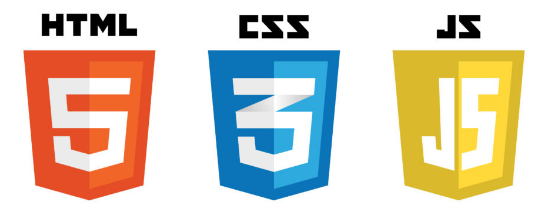
\includegraphics[width=0.4\textwidth]{pic/html-css-js.png}}
\end{frame}


\subsection{HTML:Markup 与标签}
\begin{frame}{HTML:Markup 与标签}
\begin{itemize}
    \item HTML:\textbf{H}yper\textbf{T}ext \textbf{M}arkup \textbf{L}anguate
    \item Markup Language:标记语言
    \begin{itemize}
        \item 文本与标记的结合
        \item 由标记实现所有的额外功能:格式、样式、数据、命令……
        \item 举例:HTML、XML、Markdown、\TeX 与 \LaTeX 、Open Office XML(OOXML)、YAML
    \end{itemize}
    \item 标签:实现标记的一种方式
    \begin{itemize}
        \item 基本构成:名称、属性、树结构
        \item 格式:\texttt{<tag attr=value> text </tag>}
        \item 基本标准:XML
    \end{itemize}
    \item 传统布局方式:\texttt{table}
\end{itemize}

\centering{
\includegraphics[width=0.15\textwidth]{pic/coding.png}}
\end{frame}

\subsection{网页布局}
\begin{frame}{网页布局}
\begin{block}{\faCode\ \texttt{my-first-document.html}}
利用 HTML 布局自己的博客首页。
\end{block}

\pause
\begin{itemize}
    \item 文件分块:\texttt{html -> head, body}
    \item 元数据(metadata):\texttt{meta}、\texttt{title}(与显示的「标题」区分)
    \item 基本容器:\texttt{div}
    \item \texttt{id} 与 \texttt{class}:个人与集体
    \item 常见框架:\texttt{container}、\texttt{header}、\texttt{main}、\texttt{footer}
    \item 常用标签:\texttt{p} 与 \texttt{span}、\texttt{h}\emph{n}、\texttt{ul/ol}
    与 \texttt{li}、\texttt{blockquote}、\texttt{strong} 与 \texttt{emph}、\texttt{hr}
    \item 超文本内容:\texttt{img}、\texttt{a}
\end{itemize}
\end{frame}

\subsection{CSS 样式表}
\begin{frame}{CSS 样式表}
\begin{block}{\faCode\ \texttt{style.css}}
「发明」一份修改样式的代码。
\end{block}

\pause
\begin{itemize}
    \item CSS(\textbf{C}ascading \textbf{S}tyle \textbf{S}heets):层叠样式表
    \begin{itemize}
        \item 特性:样式、层叠(按优先级覆盖)
        \item 布局、美化、动态效果等均可实现
    \end{itemize}
    \item 语法:
    \begin{itemize}
        \item 基本规则:\texttt{selector \{prop:value;\} }
        \item 选择器语法:\texttt{\#id}、\texttt{.class}、继承、通配
    \end{itemize}
    \item 元素级定义、嵌入定义与独立文件
    \item 利用浏览器「开发者工具」进行测试
    \item 「新」动向:Less、Sass/SCSS、Stylus
\end{itemize}
\end{frame}

\subsection{脚本与交互:JavaScript}
\begin{frame}{脚本与交互:JavaScript}
\begin{block}{\faCode\ \texttt{test.js}}
生成一个最简单的 JavaScript 交互脚本,并嵌入网页。
\end{block}

\pause
\begin{itemize}
    \item 脚本语言:「解释性」、「批处理」、「易学易用」、「自动化工具」
    \item 举例:JavaScript、xx-sh、CMD、MATLAB、Lua、Perl、Ruby、Python
    \item 独立实现动态功能
    \item 「新」动向:
    \begin{itemize}
        \item JQuery:简单易用,功能强大的「查询器」
        \item 前端框架:React、Angular、Bootstrap
        \item 服务端运行:Node.js(通用化)
        \item 新的模式:CoffeScript、TypeScript 等
        \item 未来……
    \end{itemize}
\end{itemize}
\end{frame}

\section{为何 Markdown}
\begin{frame}{为何 Markdown}{Markdown 是一种 Markup}
\begin{itemize}
    \item 「常年使用 HTML 撰写文档和作业」
    \item 对基本元素的取舍:移除可拓展性,简化标记语法
    \begin{itemize}
        \item 各类标签的常用子集:文档「八大金刚」
        \begin{itemize}
            \item 段落、粗斜体
            \item 标题、引用块、列表、分割线
            \item 图片、超链接
        \end{itemize}
        \item 从标签到单字符标记
        \item 构建到 HTML 的一个单射
    \end{itemize}
    \item Markdown:降低工作量,提高效率
\end{itemize}

\begin{alertblock}{结论一}
Markdown 是目前最易于使用的文本标记(Markup)语言,没有之一。
\end{alertblock}
\end{frame}

\subsection{设计哲学}
\begin{frame}{设计哲学}
\begin{block}{What is Markdown?}
Markdown is a text-to-HTML conversion tool for web writers. Markdown allows you
to write using an \textbf{easy-to-read}, \textbf{easy-to-write} plain text format,
then convert it to structurally valid XHTML (or HTML).

\raggedleft --- John Gruber
\end{block}

\begin{itemize}
    \item 可读性与可写性并重:既好看,又好写
    \item 纯文本,面向 HTML 格式
    \item 允许用 HTML 标签引入额外功能
    \item 文本多于标记
    \item \textbf{内容与样式分离}:继承自 HTML
\end{itemize}

\end{frame}

\subsection{基本语法}
\begin{frame}[fragile]
\frametitle{基本语法}\scriptsize
\begin{block}{Markdown Cheat Sheet}
\begin{verbatim}
# Markdown 简介
Markdown 是一种<u>文本标记语言</u>,用于转化为 HTML 文档。

## 功能介绍
它可以实现以下功能:

1. 对文本的**加粗**或*斜体*处理;
2. 实现不同层级的标题;
3. 标记[超链接](https://qyxf.site);
4. 插入图片,如![精彩图片](https://qyxf.site/beautiful-girl.jpg);

其支持的列表包括:

* 有序列表(ordered list)
* 无序列表(unordered list)

---

> 除此以外,Markdown 还可以实现引用块、分割线等功能。
\end{verbatim}
\end{block}
\end{frame}

\subsection{解析与渲染:搭建个人网站}
\begin{frame}{解析与渲染:搭建个人网站}\scriptsize
\vspace{\baselineskip}

\pause
\begin{block}{HTML 的来源}
\begin{itemize}
    \item 撰写 Markdown 文档,用编译器转换为 HTML 文档。
    \item 预制 HTML 模板,转换 YAML 头信息,增强效果。
\end{itemize}
\end{block}

\pause
\begin{block}{CSS 的来源}
\begin{itemize}
    \item 手写 CSS:「世上无难事,只要肯折腾」。
    \item 「标准化表格」基础上用 Less、Sass 等加快撰写进度。
    \item 直接使用他人预制的主题,或在其上做微小改动。
\end{itemize}
\end{block}

\pause
\begin{block}{JavaScript 的来源}
\begin{itemize}
    \item 需求推动学习 JavaScript 和 JQuery;不要也罢。
    \item 不重造轮子(因为不会),直接应用开源成果。
\end{itemize}
\end{block}

\pause
\begin{alertblock}{一体化解决方案}
博客渲染工具:Jekyll、Hugo、Hexo……
\end{alertblock}

\end{frame}

\subsection{Markdown 方言}

\end{document}


